Let $I$ be the incenter of a non-isosceles triangle $ABC$. Let $F$ be the intersection of the perpendicular to $AI$ through $I$ with $BC$. Let $M$ be the point on the circumcircle of $ABC$ such that $MB=MC$ and such that $M$ is on the same side of the line $BC$ as $A$. Let $N$ be the second intersection of the line $MI$ with the circumcircle of $BIC$. Prove that $FN$ is tangent to the circumcircle of $BIC$.

\textbf{Solution 1}
D'abord, on définit $D$ la deuxième intersection de $AI$ avec le cercle circonscrit du triangle $ABC$. Par le théorème incenter/excenter, $D$ est le centre du cercle circonscrit de $BIC$. Puisque $\angle FID = 90$, on déduit que $FI$ est tangent à ce cercle. Ainsi, si l'on prouve $FI = FN$, on aura terminé. De manière équivalente, étant donné que $DI = DN$ ($D$ est le centre du cercle), il suffit de prouver que $FD$ est perpendiculaire à $IN$. Définissons $P$ comme le point sur $IN$ tel que $\angle DPI = 90$. Notre but: montrer que $D,P,F$ sont alignés. On obtient alors $\angle DPM = 90$, et puisque $DM$ est un diamètre du cercle circonscrit au triangle $ABC$, $P$ se trouve alors sur ce cercle. Etant donné que $\angle DPI = 90$, le centre du cercle circonscrit de $DPI$ est le milieu du segment $ID$. Donc, $FI$ est tangent à ce cercle. On a maintenant trois cercles: les cercles circonscrits aux triangles $ABC$, $BIC$ et $PID$. Il est connu que les trois lignes de puissance de chaque paire de cercles se croisent en un point. Ce point est $F$, et puisque $DP$ est la ligne de puissance des cercles circonscrits à $DIP$ et $ABC$, alors $D,P,F$ sont alignés.

\begin{figure}[h!]
    \centering
    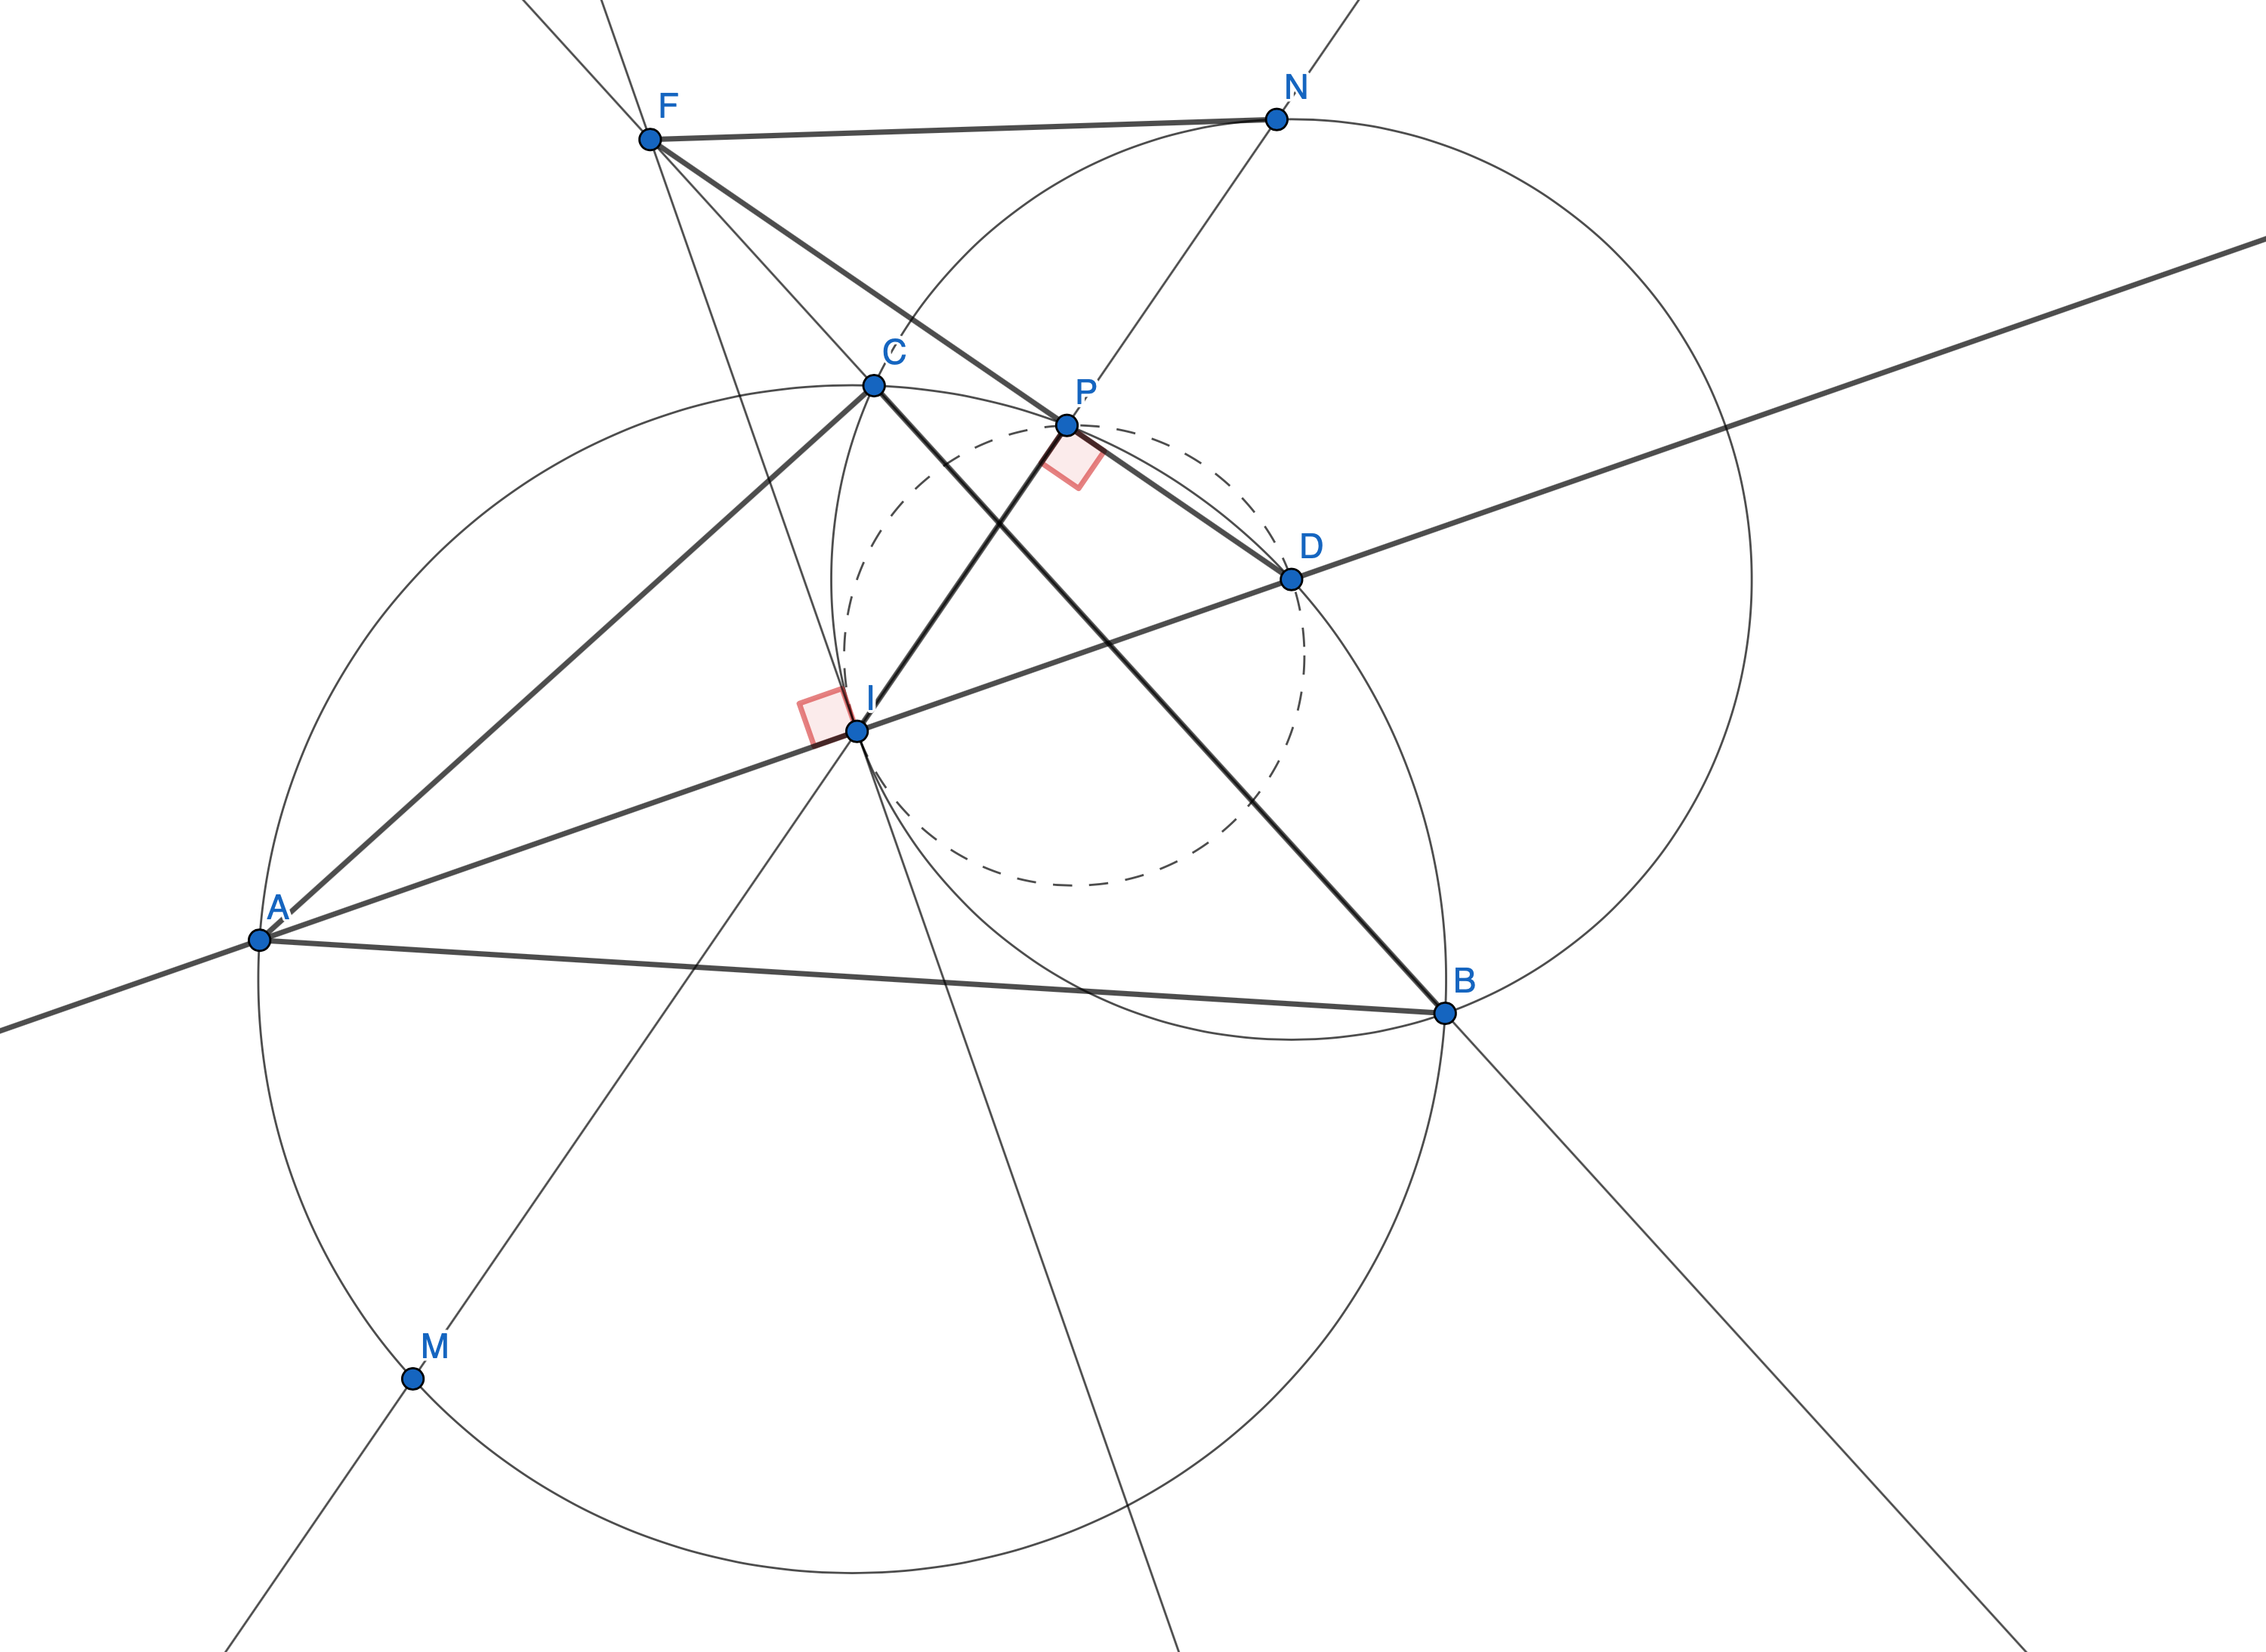
\includegraphics[width = 0.7\textwidth]{solutions/P8_1.png}
    \caption{First solution}
\end{figure}

\textbf{Marking Scheme}

\begin{itemize}
\item 1P: Introduce $D$ and explicitely say that $D$ is the center of the circumcircle of $BIC$.
\item 1P: Explicity state that $FI$ is tangent to that circle.
\item 1P: Introduce $P$ and prove that $P$ is on the circumcircle of $ABC$.
\item 3P: Prove that $D,P,F$ are collinear.
\item 1P: Conclude.
\end{itemize}

\newpage

\textbf{Solution 2}
Comme dans la solution précédente, on pose $D$ comme le milieu de l'arc $BC$. Soit également $Q$ le milieu du segment $BC$. Nous pouvons voir que $DM$ est un diamètre du cercle circonscrit à $ABC$. Du plus, $Q \in [DM]$. Donc, $\angle DBM = 90$ et les triangles $MQB$ et $MBD$ sont similaires. Alors $MB^2 = MQ \cdot MD$. Aussi, MB est tangent au cercle circonscrit au triangle $BIC$. Donc $MB^2 = MI \cdot MN$. Alors $MI \cdot MN = MQ \cdot MD$ et les points $D,Q,I,N$ sont cocyliques. De plus, $\angle FQD = 90 = \angle FID$ et $F$ se trouve également sur ce cercle. Il s'ensuit directement que $\angle FND = 90$ et donc que $FN$ est tangente au cercle circonscrit de $BIC$.
\begin{figure}[h!]
    \centering
    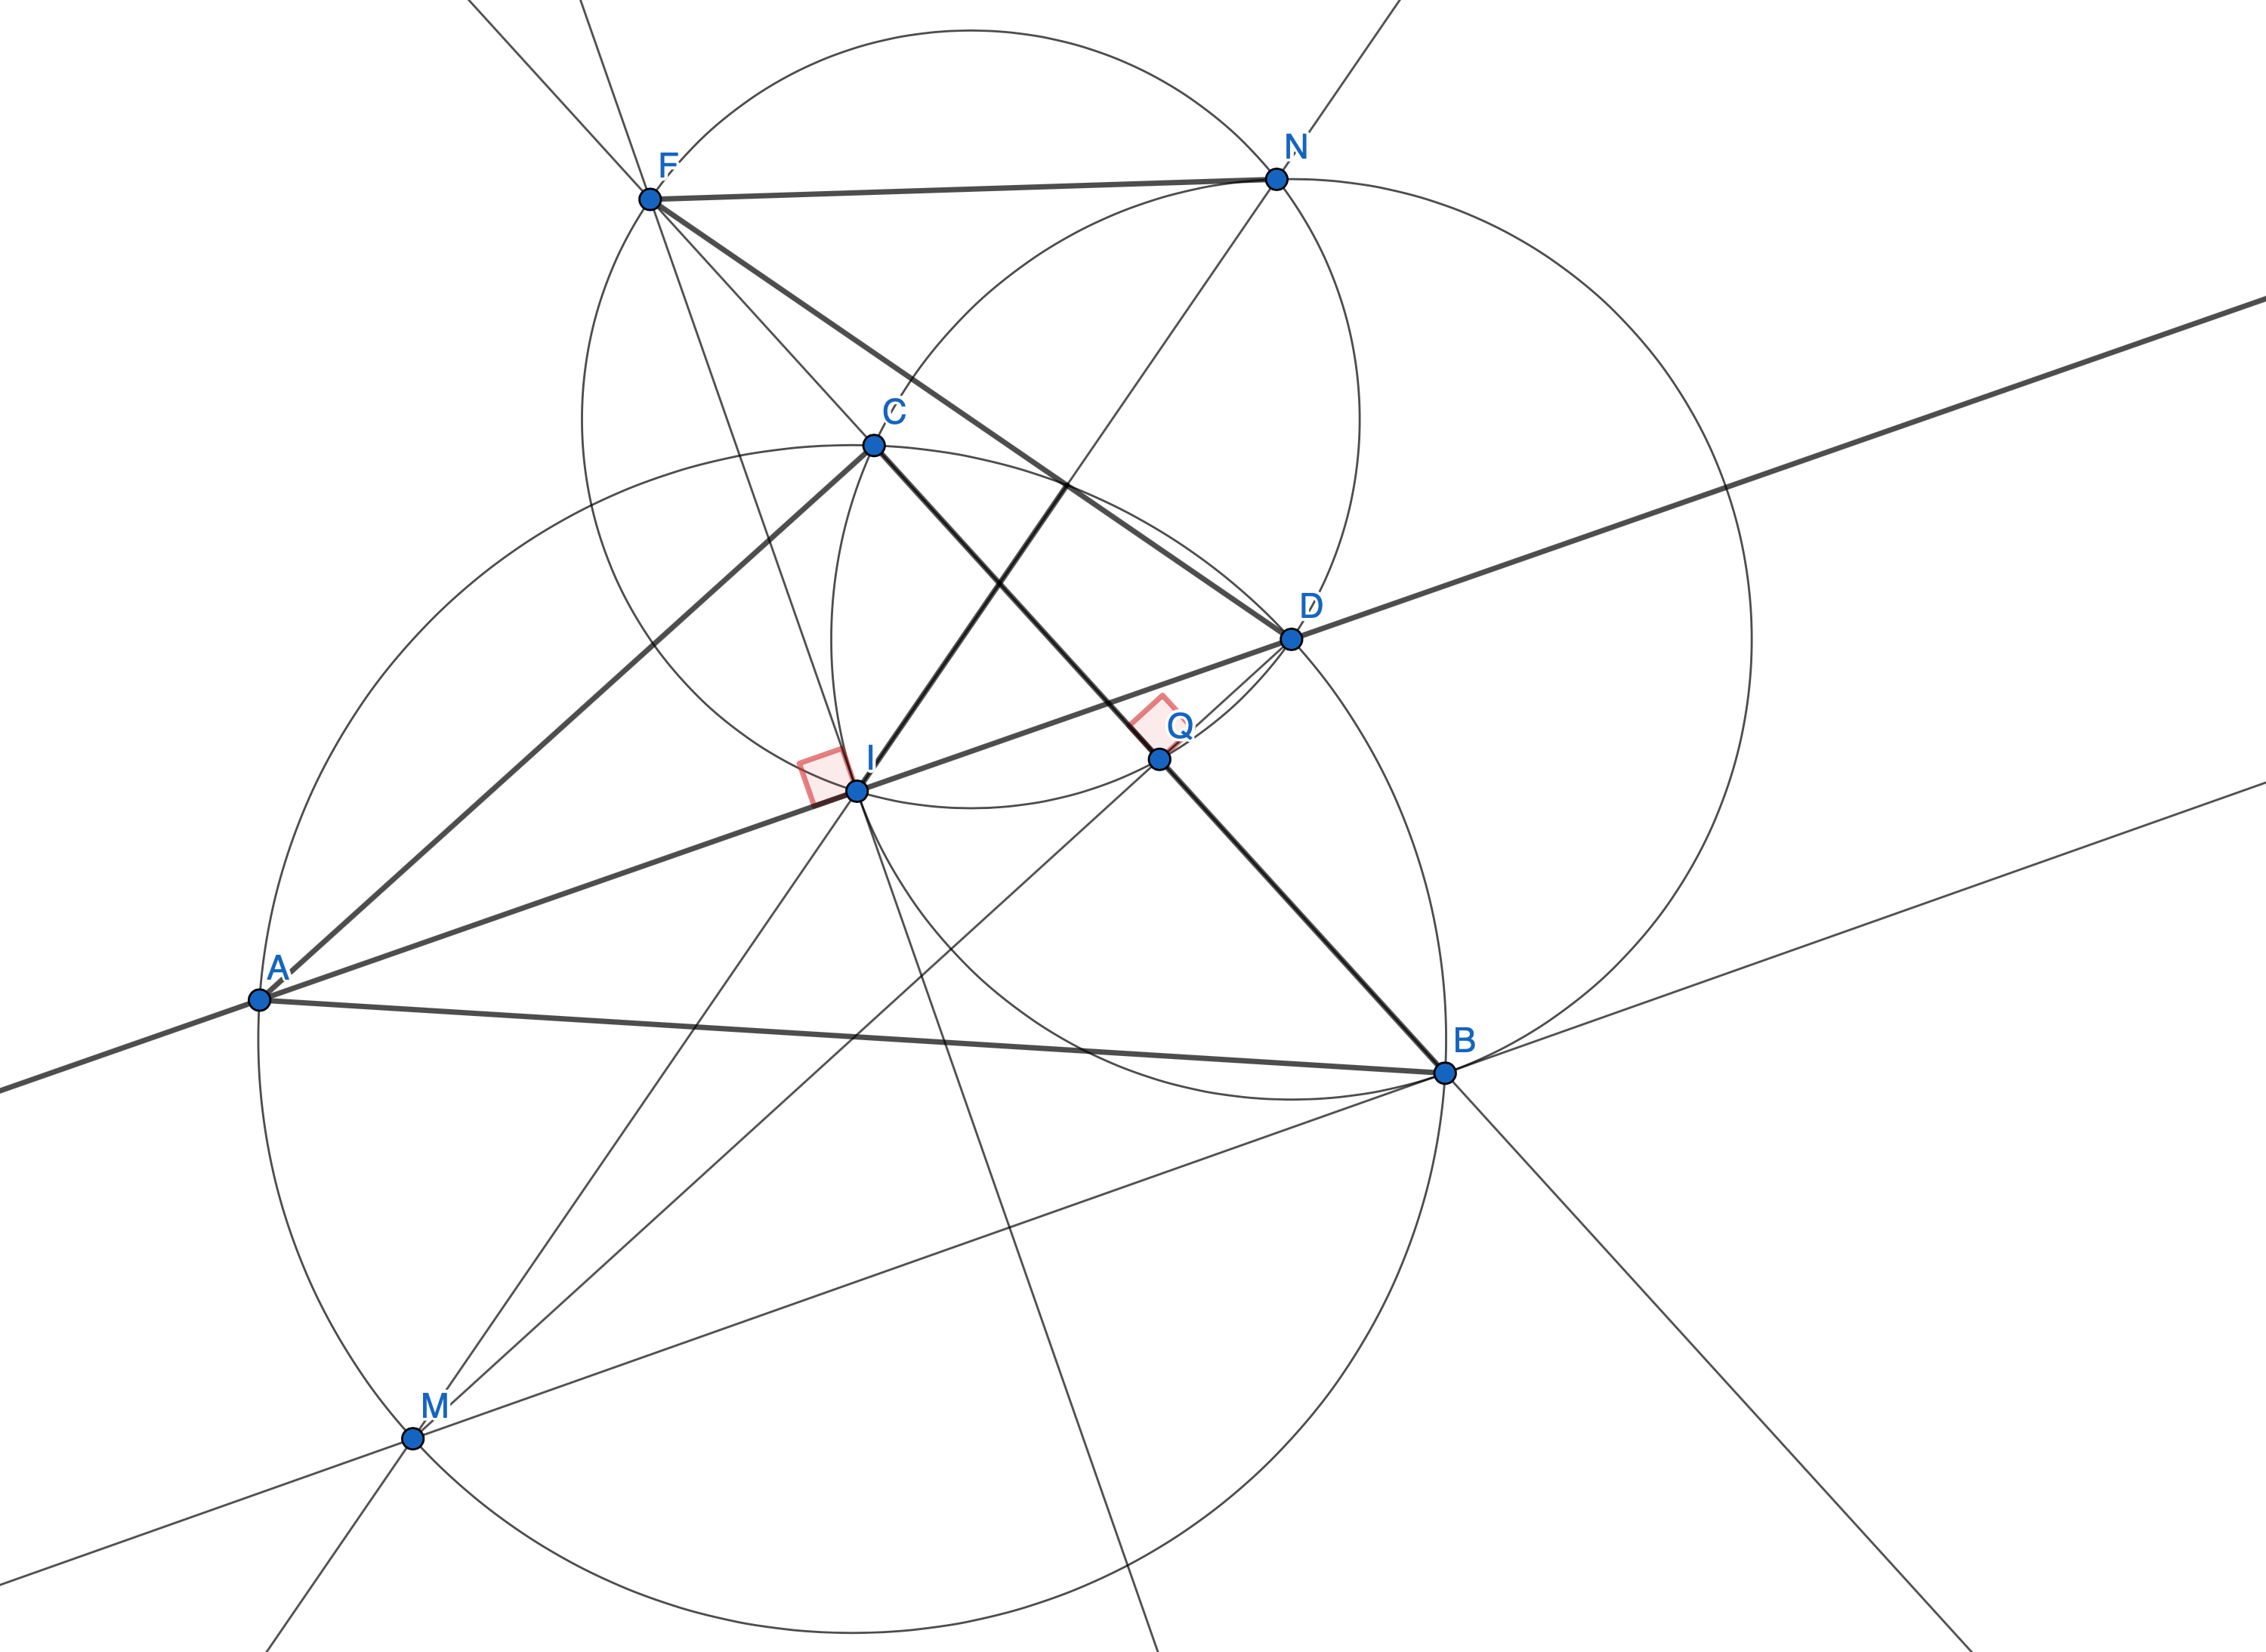
\includegraphics[width = 0.7\textwidth]{solutions/P8_2.png}
    \caption{Second solution}
\end{figure}

\textbf{Marking Scheme} 

\begin{itemize}
\item 1P: Introduce $D$ and explicitly say that $D$ is the centre of the circumcircle of $BIC$.
\item 1P: Explicitely state that $MB$ (or $MC$) is tangent to the circumcircle of $BIC$.
\item 2P: Introduce point $Q$ and use similar triangles to obtain $MB^2 = MQ \cdot MD$.
\item 1P: Use the power of point $M$ and get $MB^2 = MI \cdot MN$ and prove that $N,D,Q,I$ are concyclic.
\item 1P: Prove that $F$ is also on the circle.
\item 1P: Conclude.

\end{itemize}
